
\section{Omitted Proofs}
\subsection{Proof of Theorem \ref{the: bcd subproblem}} \label{app: monotonicity proof}
We start by proving the closed-form solution \eqref{eq: bcd_closed_form_subproblem_u}, noting that the proof for \eqref{eq: bcd_closed_form_subproblem_v} follows the same reasoning.
The objective function in the subproblem \eqref{eq: bcd subproblem: u} can be reformulated as follows:
\begin{align}
    \argmin_{\bm{u}_r \in \Z_{[\alpha,\beta]}^M} \|\bm{E}_r - \bm{u}_r \bm{v}_r^\mathsf{T}\|_{\rm F} 
    = \argmin_{\bm{u}_r \in \Z_{[\alpha,\beta]}^M}\sum_{i=1}^M \sum_{j=1}^N (e_{ij}^r - u_i^r v_j^r)^2,
    \label{eq: bcd subproblem: u: reform}
\end{align}
where $e_{ij}^r$ denotes the element of matrix $\bm{E}_r$ in the $i$th row and $j$th column, and $u_i^r$ and $v_j^r$ are the $i$th and $j$th elements of vectors $\bm{u}_r$ and $\bm{v}_r$, respectively. Since the elements of $\bm{E}_r$ and $\bm{v}_r$ are fixed in problem \eqref{eq: bcd subproblem: u}, the optimization \eqref{eq: bcd subproblem: u: reform} can be decoupled into $M$ optimizations as follows:
\begin{align}
    \argmin_{u^r_i \in \Z_{[\alpha,\beta]}} & ~q_i(u_i^r), \quad \forall i\in\{1,\dots,M\}, \nonumber\\
    \textstyle \text{where} ~~ &q_i(u_i^r) \coloneqq \sum_{j=1}^N (e_{ij}^r - u_i^r v_j^r)^2.
    \label{eq: bcd subproblem: u: decoupled}
\end{align}
The objective functions $q_i(u_i^r)$ in \eqref{eq: bcd subproblem: u: decoupled} are single-variable quadratic problems. Hence, the global optimum in each decoupled optimization problem can be achieved by finding the minimum of each quadratic problem and then projecting it onto the set $\Z_{[\alpha,\beta]}$. The minimum of each quadratic function in \eqref{eq: bcd subproblem: u: decoupled}, denoted by $\bar{u}_i^r$, can be simply found by
\begin{align}
    \textstyle \nabla_{u_i^r} q_i(u_i^r) = 0 \implies \bar{u}_i^r = \nicefrac{\sum_{j=1}^N e_{ij}^r v_j^r}{\sum_{j=1}^N v_j^{r^2}},
    \label{eq: bcd subproblem: u: minimum}
\end{align}
where $\nabla_x$ is the partial derivative with respect to $x$.
Since $q_i$ has a constant curvature (second derivative) and $q_i(\bar{u}_i^r + d)$ is nondecreasing with increasing $|d|$, the value in the set $\Z_{[\alpha,\beta]}$ which is closest to $\bar{u}_i^r$ is the global minimizer of \eqref{eq: bcd subproblem: u: decoupled}. This value can be reached by projecting $\bar{u}_i^r$ onto the set $\Z_{[\alpha,\beta]}$, namely $u^{r^\star}_i = \clamp_{[\alpha,\beta]}(\round(\nicefrac{\sum_{j=1}^N e_{ij}^r v_j^r}{\sum_{j=1}^N v_j^{r^2}}))$, which is presented for all $i\in\{1,...,M\}$ in a compact form in \eqref{eq: bcd_closed_form_subproblem_u}.



\subsection{Proof of Theorem \ref{thm:convergence}} \label{app: convergence proof}

To study the convergence of the proposed Algorithm \ref{alg: bcd for imf}, we recast the optimization problem \eqref{eq: imf problem} to the following equivalent problem:
\begin{align}
    \begin{split}
        \minimize_{U_{:r} \in \R^{M}, V_{:r} \in \R^{N}, \forall r\in\{1,...,R\}} \Psi(\bm U, \bm V) &\coloneqq f_0(\bm U, \bm V) + \sum_{r=1}^R f_r(U_{:r}) + \sum_{r=1}^R g_r(V_{:r}),\\
        \text{where} \quad~~~ f_0(\bm U, \bm V) &\coloneqq \|\bm X - \bm U \bm V^{\rm T} \|_{\rm F}^2,\\
        f_r(U_{:r}) &\coloneqq \delta_{[a,b]}(U_{:r}) + \delta_\Z(U_{:r}),\\
        g_r(V_{:r}) &\coloneqq \delta_{[a,b]}(V_{:r}) + \delta_\Z(V_{:r}),
    \end{split}
    \label{eq: IMF_surrogate}
\end{align}
with $\delta_\mathcal{B}(\cdot)$ as the indicator function of the nonempty set $\mathcal{B}$ where $\delta_\mathcal{B}(\bm x) = 0$ if $\bm x \in \mathcal{B}$ and $\delta_\mathcal{B}(\bm x) = +\infty$, otherwise. By the definition of functions above, it is easy to confirm that the problems \eqref{eq: imf problem} and \eqref{eq: IMF_surrogate} are equivalent.

The unconstrained optimization problem \eqref{eq: IMF_surrogate} consists of the sum of a differentiable (smooth), convex function $f_0$ with nonsmooth, nonconvex functions $f_r$ and $g_r$. This problem has been extensively studied in the literature under the class of nonconvex nonsmooth minimization problems.
One of the common algorithms applied to such a problem class is the well-known forward-backward-splitting (FBS) algorithm \cite{combettes2011proximal,bauschke2017correction}.
In Algorithm \ref{alg: bcd for imf}, the blocks $U_{:r}$ and $V_{:r}$ are updated sequentially following block coordinate (BC) descent minimization algorithms, also often called Gauss-Seidel updates or alternating minimization \cite{nesterov2012efficiency,attouch2013convergence}.
Hence, in this convergence study, we are interested in algorithms that allow BC-type updates for the nonconvex nonsmooth problem of \eqref{eq: IMF_surrogate} \cite{beck2013convergence,bolte2014proximal}. Specifically, we focus on the proximal alternating linearized minimization (PALM) algorithm \cite{bolte2014proximal}, to relate its convergence behavior to that of Algorithm \ref{alg: bcd for imf}.
To that end, we show that the updates of Algorithm \ref{alg: bcd for imf} are equivalent to the updates of PALM on the recast problem of \eqref{eq: IMF_surrogate}, and all the assumptions necessary for the convergence of PALM are satisfied by our problem setting.

The PALM algorithm can be summarized as follows:
\begin{enumerate}
    \item Initialize $\bm U^{\rm init} \in \R^{M\times R}$, $\bm V^{\rm init} \in \R^{N\times R}$ 
    \item For each iteration $k=0,1,...$ 
    \begin{align}
        \begin{split}
            \mysubnumber\quad \bm U^{k+1} &\in \prox^f_{c_k} \left(\bm U^k - \frac{1}{c_k} \nabla_{\bm U} H(\bm U^k, \bm V^k)\right), ~\text{with}~ c_k > L_1(\bm V^k)\\
            \mysubnumber\quad \bm V^{k+1} &\in \prox^g_{d_k} \left(\bm V^k - \frac{1}{d_k} \nabla_{\bm V} H(\bm U^{k+1}, \bm V^k)\right), ~\text{with}~ d_k > L_2(\bm U^{k+1})
        \end{split}
        \label{eq: palm_updates}
    \end{align}
\end{enumerate}
where the proximal map for an extended proper lower semicontinuous (nonsmooth) function $\func{\varphi}{\R^n}{(-\infty,+\infty]}$ and $\gamma > 0$ is defined as $\prox^\varphi_\gamma(\bm x) \coloneqq \argmin_{\bm w\in\R^n}\left\{\varphi(\bm w) + \frac{\gamma}{2} \|\bm w - \bm x\|^2_2\right\}$, and $L_1 > 0$, $L_2 > 0$ are local Lipschitz moduli, defined in the following proposition.
It is also remarked that the iterates in \eqref{eq: palm_updates} can be extended to more than two blocks, which is our case in Algorithm \ref{alg: bcd for imf} with a block representing a column of $\bm U$ or $\bm V$, without violation of the convergence. However, for the sake of presentation, we study these BC-type iterates with two blocks of the form \eqref{eq: palm_updates}. 

The following proposition investigates the necessary assumptions (cf. \cite[Asm. 1 and Asm. 2]{bolte2014proximal}) for convergence iterates in \eqref{eq: palm_updates}.
\begin{prop}[Meeting required assumptions]\label{prop: assumptions}
    The assumptions necessary for the convergence of iterates in \eqref{eq: palm_updates} are satisfied by the functions involved in the problem \eqref{eq: IMF_surrogate}, specifically:
    \begin{enumerate}
        \item The indicator functions $\delta_{[a,b]}$ and $\delta_\Z$ are proper and lower semicontinuous functions, so do the functions $f$ and $g$;
        \item For any fixed $\bm V$, the partial gradient $\nabla_{\bm U} H(\bm U, \bm V)$ is globally Lipschitz continuous with modulus $L_1(\bm V) = \|\bm V^T \bm V\|_{\rm F}$ defined by
        \begin{equation*}
            \|\nabla_{\bm U} H(\bm U_1, \bm V) - \nabla_{\bm U} H(\bm U_2, \bm V)\| \leq L_1(\bm V) \|\bm U_1 - \bm U_2\|, \quad \forall \bm U_1,\bm U_2 \in \R^{M\times R},
        \end{equation*}
        where $\|\cdot\|$ in this section denotes the $\ell_2$-norm of the vectorized input with the proper dimension (here, with the input in $\R^{MR\times 1}$).
        The similar Lipschitz continuity is evident for $\nabla_{\bm V} H(\bm U, \bm V)$ as well with modulus $L_2(\bm U) = \|\bm U \bm U^T\|_{\rm F}$.
        \item The sequences $\bm U^k$ and $\bm V^k$ are bounded due to the indicator functions $\delta_{[a,b]}$ with bounded $a$ and $b$. Hence the moduli $L_1(\bm V^k)$ and $L_2(\bm U^k)$ are bounded from below and from above for all $k\in\N$.
        \item The function $H$ is twice differentiable, hence, its full gradient $\nabla H(\bm U,\bm V)$ is Lipschitz continuous on the bounded set $\bm U \in [a,b]^{M\times R}$, $\bm V \in [a,b]^{N\times R}$. Namely, with $M > 0$:
        \begin{align}
            \begin{split}
                \|(\nabla_{\bm U} H(\bm U_1, \bm V_1) - \nabla_{\bm U} H(\bm U_2, \bm V_2), \nabla_{\bm V} H(\bm U_1, \bm V_1) - &\nabla_{\bm V} H(\bm U_2, \bm V_2))\| \\
                &\leq M \|(\bm U_1 - \bm U_2, \bm V_1 - \bm V_2)\|,
            \end{split}
        \end{align}
        where $(\cdot,\cdot)$ denotes the concatenation of the two arguments.
        \item The sets $[a,b]$ and integer numbers are semi-algebraic; so are their indicator functions. The function $H$ is also polynomial, hence it is semi-algebraic. The sum of these functions results in a semi-algebraic function $\Psi$ in \eqref{eq: IMF_surrogate}, hence $\Psi$ is a Kurdyka-Łojasiewicz (KL) function.
    \end{enumerate}
\end{prop}
By Proposition \ref{prop: assumptions}, the optimization problem \eqref{eq: IMF_surrogate} can be solved by the BC iterates in \eqref{eq: palm_updates}, due to the following proposition:
\begin{prop}[Global convergence \cite{bolte2014proximal}]\label{prop: convergence}
    With the assumptions in proposition \ref{prop: assumptions} being met by the problem \eqref{eq: IMF_surrogate}, let $\seq{(\bm U^k, \bm V^k)}$ be a sequence generated by the BC iterates in \eqref{eq: palm_updates}. Then the sequence converges to a critical point $(\bm U^\star, \bm V^\star)$ of the problem \eqref{eq: IMF_surrogate}, where $0 \in \partial \Psi(\bm U^\star, \bm V^\star)$, with $\partial$ as the subdifferential of $\Psi$.
\end{prop}

In the following, we highlight that the iterates in \eqref{eq: palm_updates} can be implemented more simply and more efficiently by Algorithm \ref{alg: bcd for imf} for the problem of image compression. It is noted that the so-called \emph{forward} steps $\bm U^k - \frac{1}{c_k} \nabla_{\bm U} H(\bm U^k, \bm V^k)$ and $\bm V^k - \frac{1}{d_k} \nabla_{\bm V} H(\bm U^{k+1}, \bm V^k)$ in the $\prox$ operators can be replaced by the simple closed-form solutions $\nicefrac{\bm{E}_r \bm{v}_r}{\lVert \bm{v}_r \rVert^2}$ and $\nicefrac{\bm{E}_r^\mathsf{T} \bm{u}_r}{\lVert \bm{u}_r \rVert^2}$ presented in \eqref{eq: bcd_closed_form_subproblem_u} and \eqref{eq: bcd_closed_form_subproblem_v}, respectively (in the case where the iterates \eqref{eq: palm_updates} are extended to multi-block updates, each block representing one column). This is thanks to the special form of the functions $H(\cdot, \bm V^k)$ and $H(\bm U^{k+1}, \cdot)$ being quadratic functions, each having a global optimal point which ensures a descent in each forward step. 
Furthermore, the proximal operators $\prox^f_{c_k}$ and $\prox^g_{d_k}$ can efficiently be implemented by the operators $\round$ and $\clamp_{[\alpha,\beta]}$ in \eqref{eq: bcd_closed_form_subproblem_u} and \eqref{eq: bcd_closed_form_subproblem_v}. The equivalence of these steps is proven in the following lemma.

\begin{lem}[$\prox$ implementation]
    Consider the operators $\round$ and $\clamp_{[\alpha,\beta]}$ defined in \eqref{eq: bcd_closed_form_subproblem_u} and \eqref{eq: bcd_closed_form_subproblem_v}.
    % Define the following (elementwise) operators $\func{P_{[a,b]}}{\R}{\R}$, and $\func{T_\Z}{\R}{\R}$:
    % \begin{align}
    %     P_{[a,b]}(x) &\coloneqq \min\{\max\{a, x\}, b\},\\
    %     T_\Z(x) &\coloneqq \max\{\lfloor x \rfloor, \lfloor x+0.5 \rfloor\}. \label{eq:Tz}
    % \end{align}
    Then $\prox^f_{c_k}(\bm W) = \round(\clamp_{[\alpha,\beta]}(\bm W))$ and $\prox^f_{d_k}(\bm Z) = \round(\clamp_{[\alpha,\beta]}(\bm Z))$ for any $\bm W\in \R^{M\times R}$, $\bm Z\in\R^{N\times R}$, and $\round(\clamp_{[\alpha,\beta]}(\cdot))$ being an elementwise operator on the input matrices.
\end{lem}
\begin{proof}
    Define the following norms for a given matrix $\bm W \in \R^{M\times R}$:
    \begin{align*}
        \|\bm W\|_{[a,b]}^2 \coloneqq \sum_{i,j \mid a \leq \bm W_{ij} \leq b} \bm W_{ij}^2, \quad 
        \|\bm W\|_a^2 \coloneqq \sum_{i,j \mid \bm W_{ij} < a} \bm W_{ij}^2, \quad 
        \|\bm W\|_b^2 \coloneqq \sum_{i,j \mid \bm W_{ij} > b} \bm W_{ij}^2.
    \end{align*}
    Moreover, note that the $\round$ operator  can be equivalently driven by the following proximal operator:
    \begin{equation}
        \round(\bm W) = \argmin_{\bm U \in \Z^{M\times R}}\{\|\bm U - \bm W\|^2_F\}.
        \label{eq: equivalence_prox_Tz}
    \end{equation}
    The proximal operator $\prox^f_{c_k}(\bm W)$ can be rewritten as
    \begin{align*}
        \prox^f_{c_k}(\bm W) &= \argmin_{\bm U \in \R^{M\times R}}\{\delta_{[a,b]}(\bm U) + \delta_{\Z}(\bm U) + \frac{c_k}{2} \|\bm U - \bm W\|^2_F\}\\
        &= \argmin_{\bm U \in \Z_{[a,b]}^{M\times R}}\{\|\bm U - \bm W\|^2_F\}\\
        &= \argmin_{\bm U \in \Z_{[a,b]}^{M\times R}}\{\|\bm U - \bm W\|^2_{[a,b]} + \|\bm U - \bm A\|^2_a + \|\bm U - \bm B\|^2_b\}\\
        &= \argmin_{\bm U \in \Z^{M\times R}}\{\|\bm U - \bm W\|^2_{[a,b]} + \|\bm U - \bm A\|^2_a + \|\bm U - \bm B\|^2_b\}\\
        &= \argmin_{\bm U \in \Z^{M\times R}}\{\|\bm U - \clamp_{[\alpha,\beta]}(\bm W)\|^2_F\}\\
        &= \round(\clamp_{[\alpha,\beta]}(\bm W)).
    \end{align*}
    The first equality is due to the definition of $\prox$ which is equivalent to the second equality. 
    In the third equality the matrices $\bm A\in\R^{M\times R}$ and $\bm B\in\R^{M\times R}$ have elements all equal to $a$ and $b$, respectively.
    The third equality is due to the fact that replacing $\|\bm U - \bm W\|^2_a + \|\bm U - \bm W\|^2_b$ with $\|\bm U - \bm A\|^2_a + \|\bm U - \bm B\|^2_b$ has no effect on the solution of the minimization. The fourth equality is also trivial due to the involved norms in the third equality. The fifth equality can be easily confirmed by the definition of $\clamp_{[\alpha,\beta]}$. Finally, in the last equality \eqref{eq: equivalence_prox_Tz} is invoked. A similar proof can be trivially followed for $\prox^f_{d_k}(\bm Z) = \round(\clamp_{[\alpha,\beta]}(\bm Z))$ as well.
\end{proof}
Now that the equivalence of iterates \eqref{eq: palm_updates} with the simple and closed-form steps in Algorithm \ref{alg: bcd for imf} is fully established, and the assumptions required for the convergence are verified in proposition \ref{prop: assumptions} to be met by problems \eqref{eq: IMF_surrogate} and \eqref{eq: imf problem}, proposition \ref{prop: convergence} can be trivially invoked to establish the convergence of Algorithm \ref{alg: bcd for imf} to a locally optimal point of problem \eqref{eq: imf problem}.


\section{Implementation Details} \label{sec: implementation details}

\paragraph{Parameter Setup.} We used a patch size of $8 \times 8$ for patchification. The number of BCD iterations for IMF is by default set to 10 (although our ablation studies in Section \ref{sec: ablation studies} suggests that even 2 iterations may be sufficient in practice). For lossless compression of factor maps, we employed the WebP codec implemented in the Pillow library \cite{clark2015pillow}. The default factor bounds are $[-16, 15]$.

\paragraph{Evaluation.} For comparison, we experimented with the widely-used Kodak dataset \cite{kodak1993}, with 24 lossless images of 768 × 512 resolution. To assess the robustness of our proposed method, we also tested it using the CLIC 2024 validation dataset \cite{clic2024}, consisting of 30 high-resolution, high-quality images. To evaluate the rate-distortion performance, we measured the bit rate in bits per pixel (bpp) and assessed the quality of reconstructed images using the peak signal-to-noise ratio (PSNR) and structural similarity index measure (SSIM) metrics. We plotted rate-distortion (RD) curves, such as the PSNR-bpp curve, for each method to demonstrate the compression performance.

\paragraph{Baseline Codecs.} For JPEG compression, we employed the Pillow library \cite{clark2015pillow}. Our SVD-based compression baseline follows the same framework as the proposed IMF compression algorithm. However, it employs truncated SVD instead of IMF, followed by uniform quantization of the factors and lossless compression using the zlib library \cite{deutsch1996zlib}. This differs from the IMF algorithm where factors are first reshaped into factor maps and then compressed losslessly as images using WebP.

\section{More Ablation Studies}

\paragraph{Patchification.} 
In Figure \ref{fig: patch ablation psnr-vs-bpp}, patchification effect with different patch sizes is investigated.
First, it can be concluded that the considered patchification technique has a positive effect on performance since it captures the locality and spatial dependencies of neighboring pixels. Hence, IMF has more representation power to reconstruct the original pattern in each patch.
The performance on various datasets has shown that patches of size $8\times 8$ lead to the best performance. The same conclusion is evident for the Kodak dataset example presented in Figure \ref{fig: patch ablation psnr-vs-bpp}.

\paragraph{Color space.}
The compression performance of IMF is studied with two color spaces, namely RGB and YC\textsubscript{B}C\textsubscript{R}, in Figure \ref{fig: colorspace ablation psnr-vs-bpp}.
Although the compression performance remains unchanged in terms of PSNR, qualitative results reported in Figure \ref{fig: qualitative_comparison_kodim19} indicate that YC\textsubscript{B}C\textsubscript{R} color space can maintain natural colors more effectively.

\begin{figure}[t]
	\centering
	\begin{subfigure}{.45\textwidth}
		\centering
		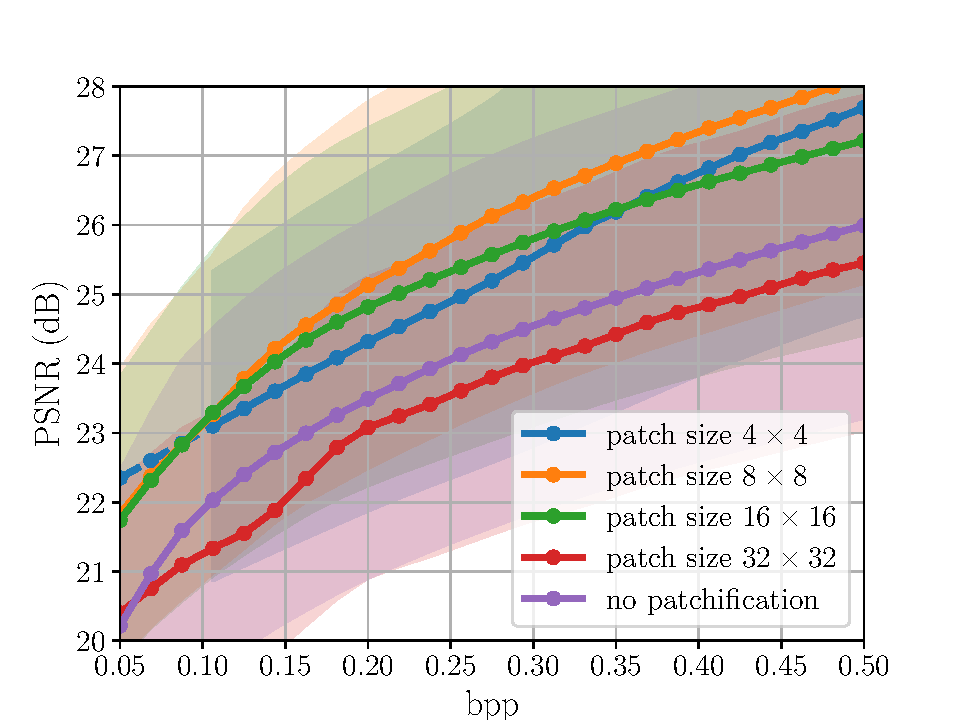
\includegraphics[width=.95\textwidth]{figures/ablation_patchsize_psnr.pdf}
		\caption{ablation on patch size}
		\label{fig: patch ablation psnr-vs-bpp}
	\end{subfigure}
    \begin{subfigure}{.45\textwidth}
		\centering
		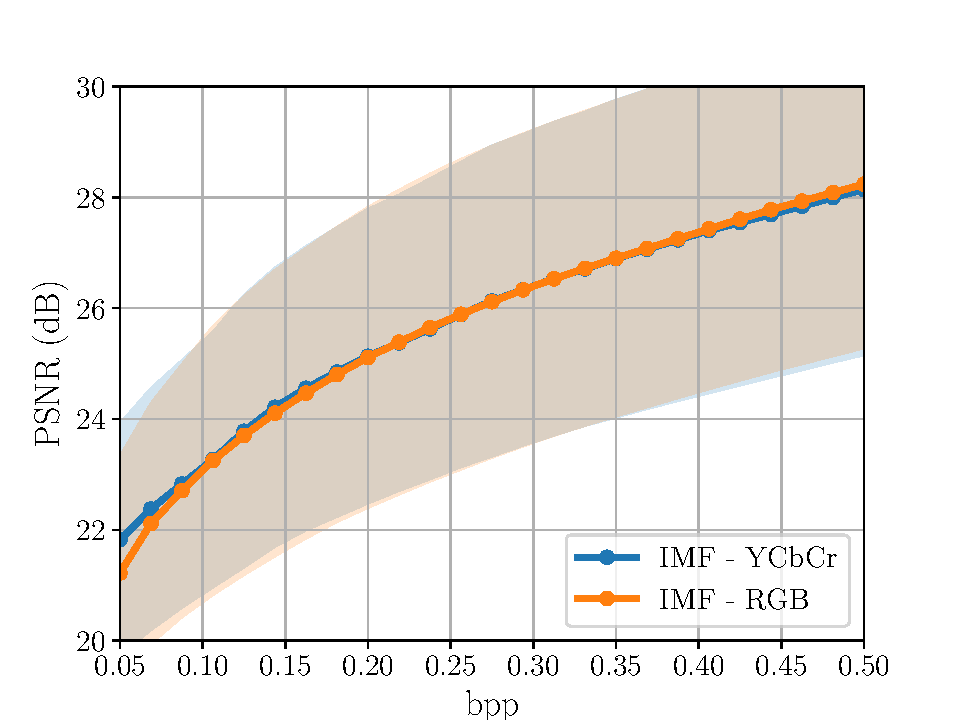
\includegraphics[width=.95\textwidth]{figures/ablation_colorspace_psnr.pdf}
		\caption{ablation on color space}
		\label{fig: colorspace ablation psnr-vs-bpp}
	\end{subfigure}%
	\caption{Ablation studies for IMF. Average PSNR on the Kodak dataset is reported versus bpp. 
    }
	\label{fig: ablation studies: appen}
\end{figure}

\begin{figure}[t]
	\centering
	\begin{subfigure}{.19\textwidth}
		\centering
        \text{\small Original image}
		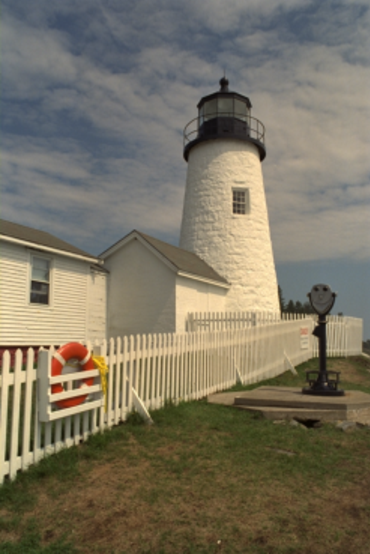
\includegraphics[trim=5cm 1.5cm 5cm 1.7cm, clip, width=1\textwidth]{figures/kodim19_original.pdf}
        \vspace{-6pt}
        \caption*{\tiny}
	\end{subfigure}%
	\begin{subfigure}{.19\textwidth}
		\centering
        \text{\small JPEG}
		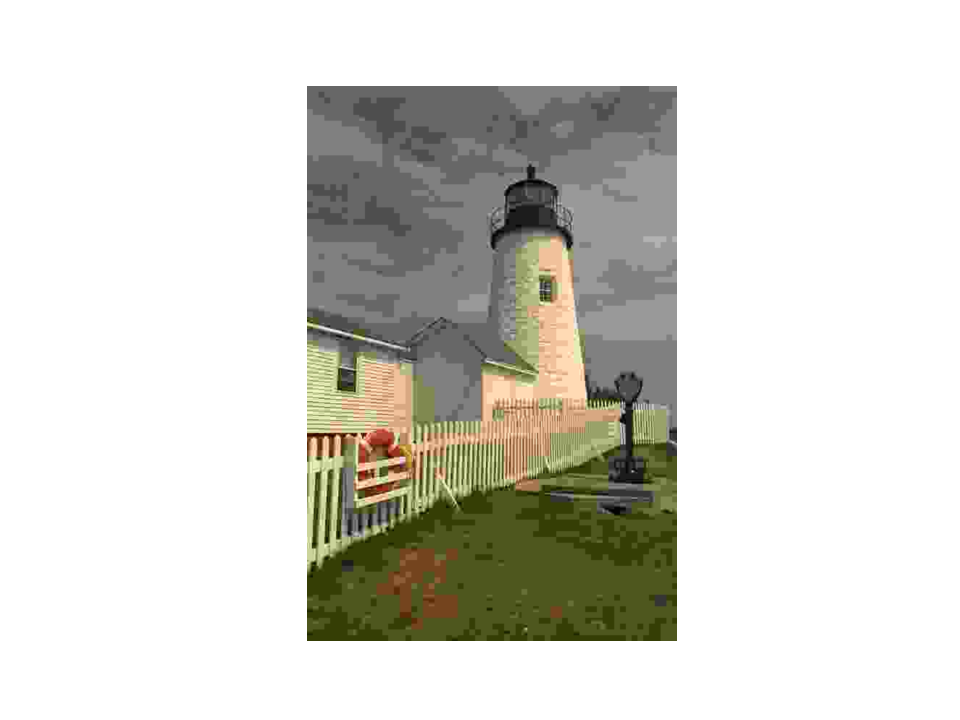
\includegraphics[trim=5cm 1.5cm 5cm 1.7cm, clip, width=1\textwidth]{figures/kodim19_JPEG_bpp_0.202.pdf}
        \vspace{-15pt}
        \caption*{\tiny \textbf{PSNR: 23.00dB \\ bpp: 0.20}}
	\end{subfigure}
    \begin{subfigure}{.19\textwidth}
		\centering
        \text{\small SVD}
		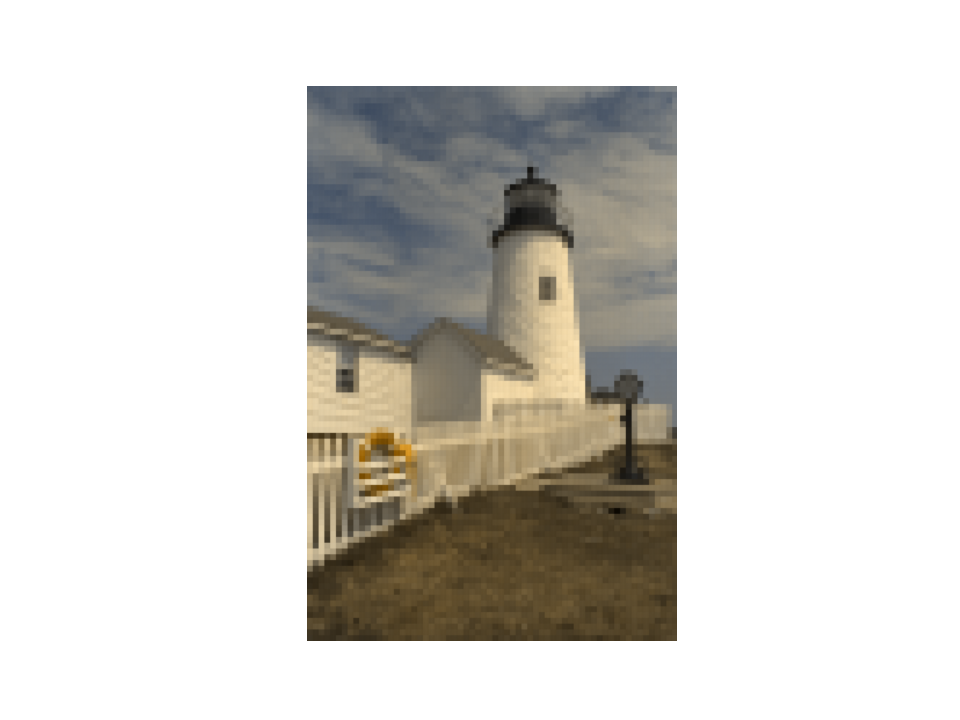
\includegraphics[trim=5cm 1.5cm 5cm 1.7cm, clip, width=1\textwidth]{figures/kodim19_SVD_bpp_0.215.pdf}
        \vspace{-15pt}
        \caption*{\tiny \textbf{PSNR: 21.53dB \\ bpp: 0.21}}
	\end{subfigure}
    \begin{subfigure}{.19\textwidth}
		\centering
		\text{\small IMF - RGB}
		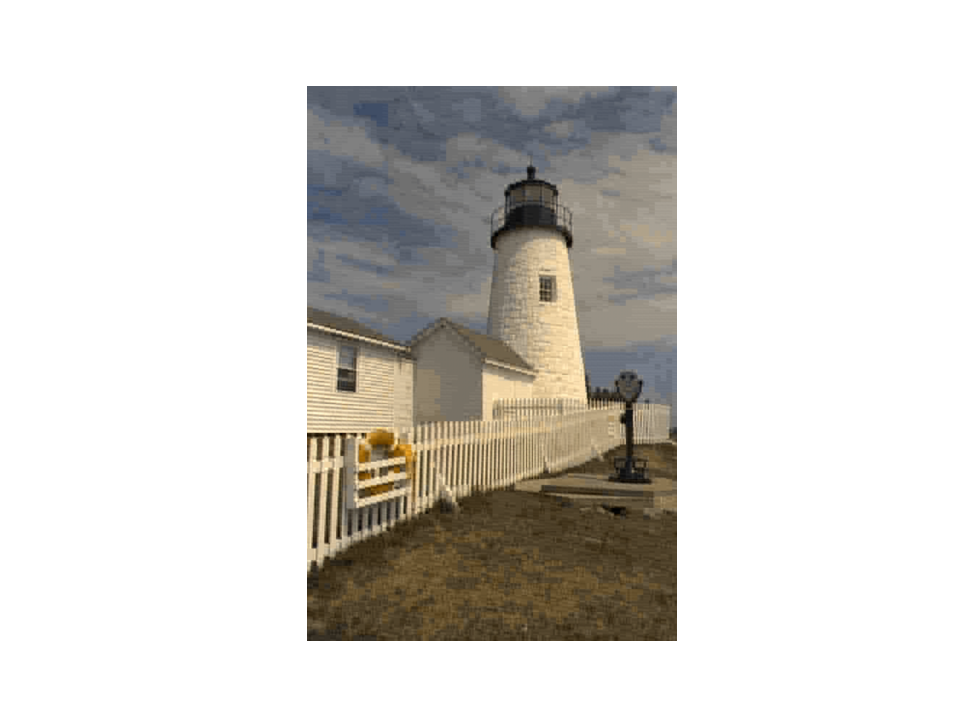
\includegraphics[trim=5cm 1.5cm 5cm 1.7cm, clip, width=1\textwidth]{figures/kodim19_IMF - RGB_bpp_0.247.pdf}
		\vspace{-15pt}
		\caption*{\tiny \textbf{PSNR: 25.40dB \\ bpp: 0.24}}
	\end{subfigure}	
    \begin{subfigure}{.19\textwidth}
		\centering
        \text{\small IMF - YC\textsubscript{B}C\textsubscript{R}}
		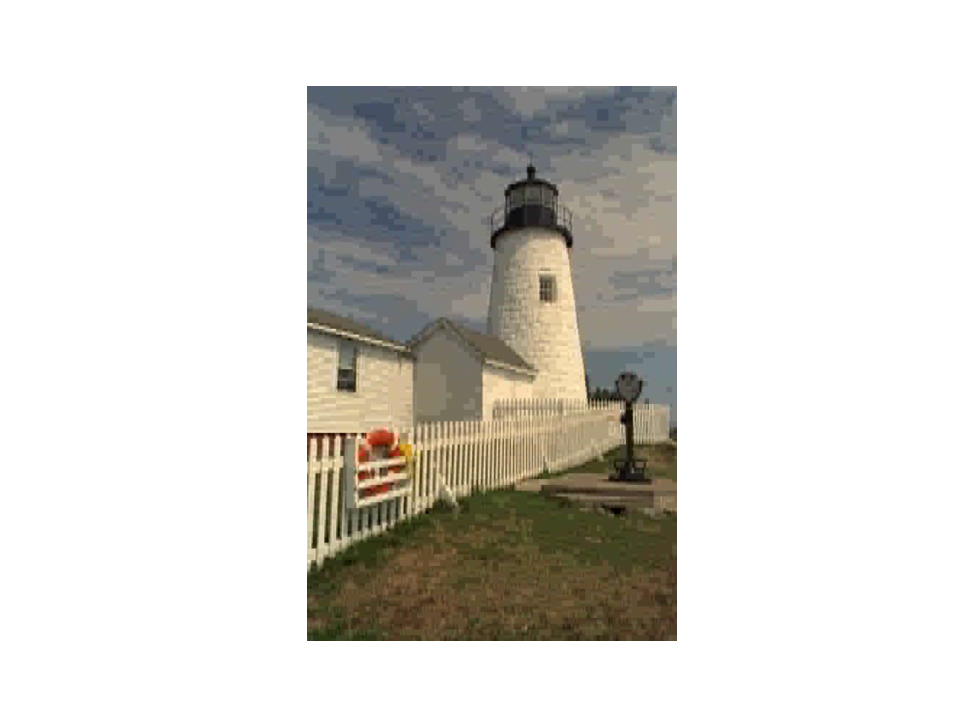
\includegraphics[trim=5cm 1.5cm 5cm 1.7cm, clip, width=1\textwidth]{figures/kodim19_IMF_bpp_0.191.pdf}
        \vspace{-15pt}
        \caption*{\tiny \textbf{PSNR: 24.32dB \\ bpp: 0.19}}
	\end{subfigure}
    \caption{Qualitative performance comparison on an image from Kodak.}
	\label{fig: qualitative_comparison_kodim19}
\end{figure}

\section{Structural Similarity Index Measure (SSIM) Metrics}
In Figures \ref{fig: compression_performance_ssim} and \ref{fig: ablation studies: ssim}, average SSIM values for the images of the Kodak and CLIC datasets are presented. 

\begin{figure}[t]
	\centering
	\begin{subfigure}{.45\textwidth}
		\centering
		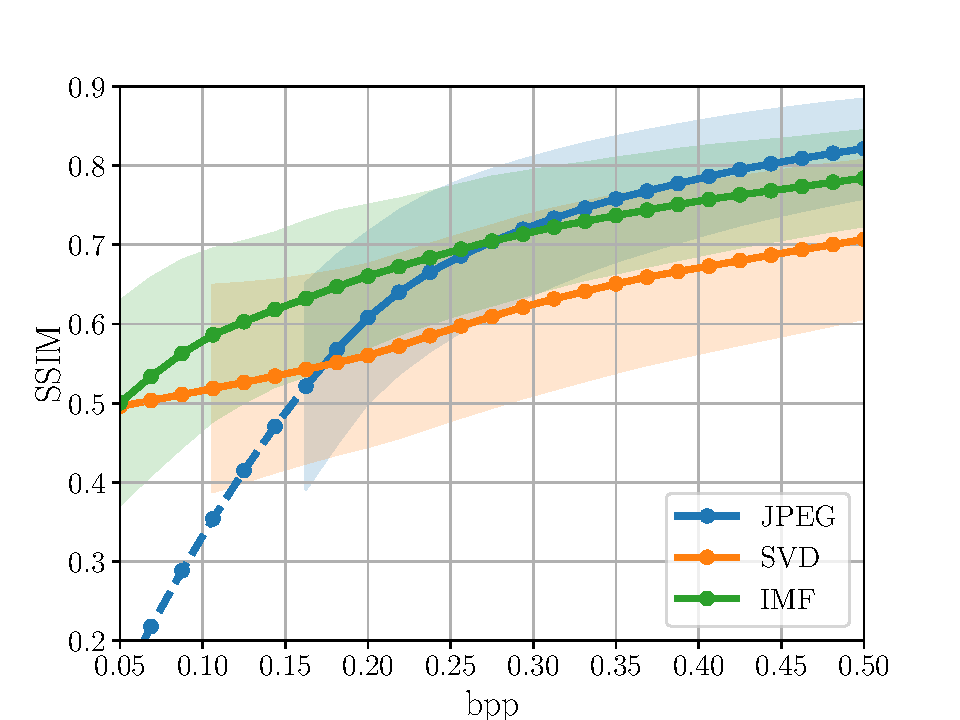
\includegraphics[width=.95\textwidth]{figures/comparison_kodak_ssim.pdf}
		\caption{Kodak}
		\label{fig: ssim-vs-bpp kodak}
	\end{subfigure}%
	\begin{subfigure}{.45\textwidth}
		\centering
		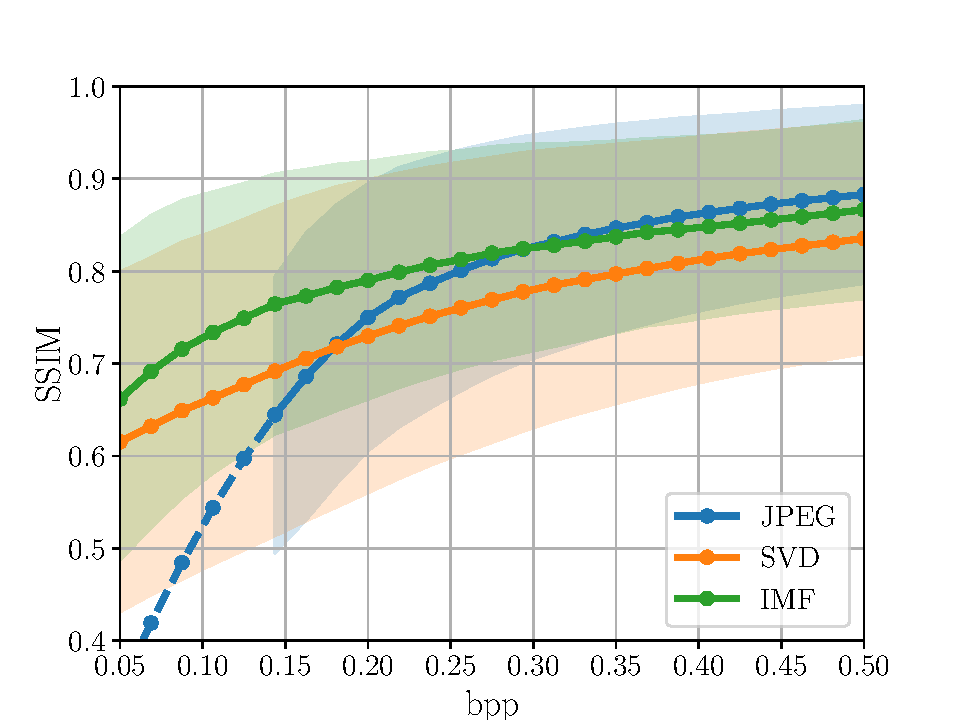
\includegraphics[width=.95\textwidth]{figures/comparison_clic_ssim.pdf}
		\caption{CLIC}
		\label{fig: ssim-vs-bpp clic}
	\end{subfigure}
	\caption{Comparison of compression algorithms on Kodak and CLIC in terms of SSIM.}
	\label{fig: compression_performance_ssim}
\end{figure}

\begin{figure}[t]
	\centering
	\begin{subfigure}{.45\textwidth}
		\centering
		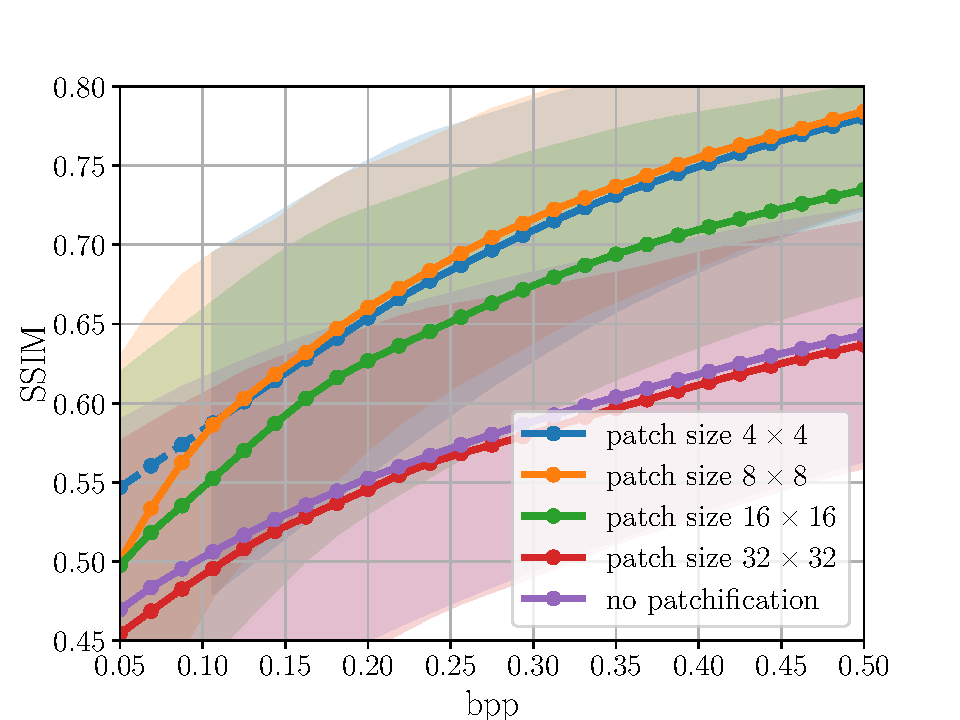
\includegraphics[width=.95\textwidth]{figures/ablation_patchsize_ssim.pdf}
		\caption{ablation on patch size}
		\label{fig: patch ablation ssim-vs-bpp}
	\end{subfigure}%
	\begin{subfigure}{.45\textwidth}
		\centering
		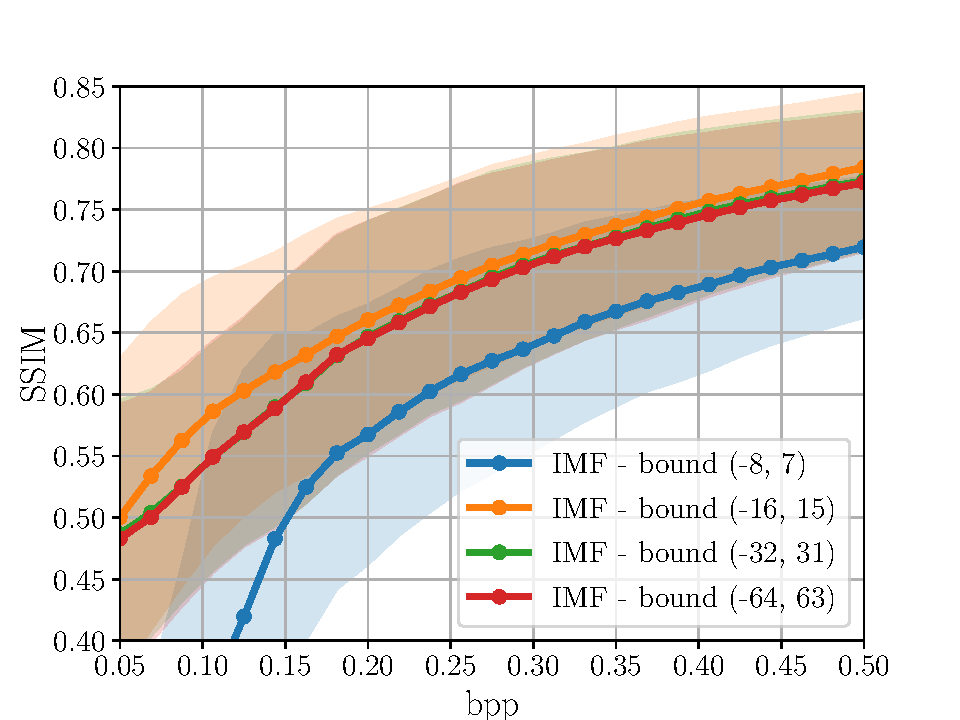
\includegraphics[width=.95\textwidth]{figures/ablation_bounds_ssim.pdf}
		\caption{ablation on factor bounds}
		\label{fig: bounds ablation ssim-vs-bpp}
	\end{subfigure}
    \begin{subfigure}{.45\textwidth}
		\centering
		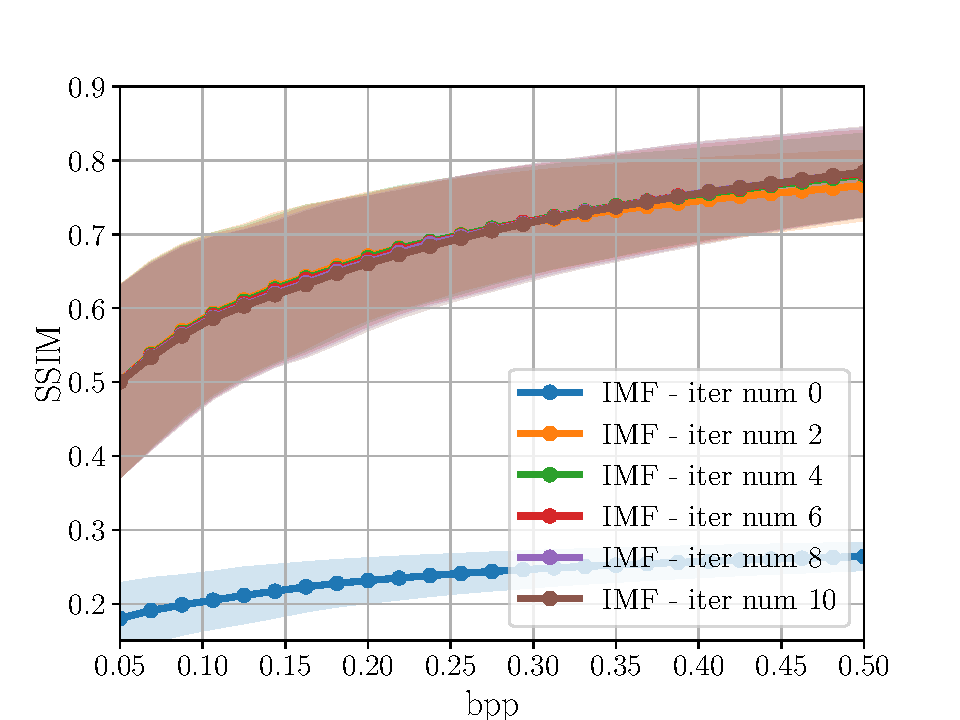
\includegraphics[width=.95\textwidth]{figures/ablation_iternum_ssim.pdf}
		\caption{ablation on BCD iteration number}
		\label{fig: iteration ablation ssim-vs-bpp}
	\end{subfigure}%
	\begin{subfigure}{.45\textwidth}
		\centering
		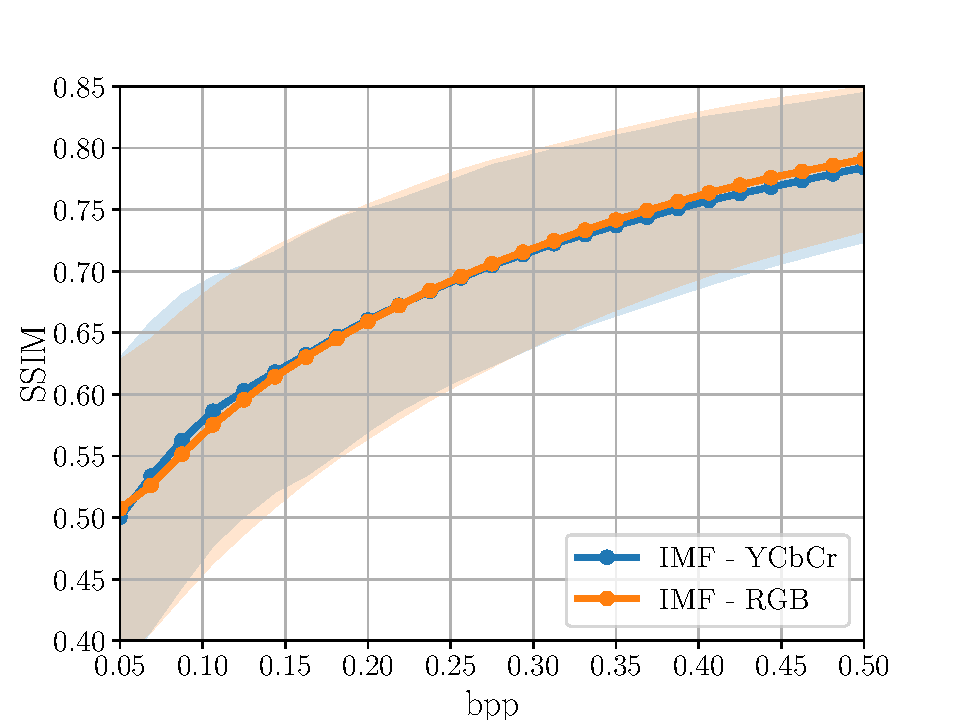
\includegraphics[width=.95\textwidth]{figures/ablation_colorspace_ssim.pdf}
		\caption{ablation on color space}
		\label{fig: colorspace ablation ssim-vs-bpp}
	\end{subfigure}
	\caption{Ablation studies for IMF. Average SSIM on the Kodak dataset is plotted as a function of bpp. 
    }
	\label{fig: ablation studies: ssim}
\end{figure}